\documentclass[12pt,a4paper]{report}
\usepackage[utf8]{inputenc}
\usepackage[english]{babel}
\usepackage{hyperref}
\usepackage{amsmath,amsfonts,amssymb}
\usepackage{verbatim}
\usepackage{bm}
\usepackage{tikz}
\usetikzlibrary{shapes,arrows}

\author{Romain Dubessy}
\title{Quantum Simulator -- Reference Manual}

\newcommand{\abs}[1]{\left|#1\right|}
\newcommand{\qsimu}{\texttt{qsimu}\,}
\newcommand{\fft}[1]{\mathcal{F}\left[#1\right]}
\newcommand{\ket}[1]{\left|#1\right>}

\renewcommand{\exp}[1]{\textrm{exp}\left[#1\right]}

\begin{document}
\maketitle
\cleardoublepage
\begin{table}
\begin{center}
\begin{tabular}{c|l}
Symbol & Definition \\\hline
$\bm{r}$ & n-dimensional vector\\
$\Delta$ & n-dimensional Laplacian\\
$t$ & Time (in physical units)\\
$m$ & Mass\\
\hline
\end{tabular}
\caption{\label{tab:notations}Some common notation used throughout this document.}
\end{center}
\end{table}
\cleardoublepage
\tableofcontents
\chapter{Introduction}
This program is designed to study the non linear Schrodinger equation (NLSE), also called Gross-Pitaevskii equation (GPE) in the cold atom community:
\begin{equation}
\imath\hbar\frac{\partial}{\partial t}\psi(\bm{r},t)=\left(-\frac{\hbar^2}{2m}\Delta+V(\bm{r},t)+gN\abs{\psi(t,\bm{r})}^2\right)\psi(\bm{r},t),
\label{eqn:gpe}
\end{equation}
white the proper normalisation $\int \bm{dr}\abs{\psi(t,\bm{r})}^2=1$.
Instead of trying to solve Eq.~\eqref{eqn:gpe} with stable algorithms that preserves the wave function normalization, which is not an obvious problem, we will make use of the formal solution of Eq.~\eqref{eqn:gpe} in term of the evolution operator:
\begin{subequations}
\begin{eqnarray}
\psi(\bm{r},t)&=&U(t,t_0)\psi(\bm{r},t_0),\\
U(t,t_0)&=&\exp{-\imath\int_{t_0}^t\frac{dt^\prime}{\hbar}\left(-\frac{\hbar^2}{2m}\Delta+V(\bm{r},t^\prime)+gN\abs{\psi(\bm{r},t^\prime)}^2\right)}.
\end{eqnarray}
\end{subequations}
This is explained in section~\ref{seq:integrator}

\section{Installation instructions}
First you need to get a working copy of the program.
The rest of the installation procedure depends on your operating system.

\subsection{Windows}

\subsection{Unix/BSD}
In the root directory issue the commands:
\begin{verbatim}
$ make
$ sudo make install
\end{verbatim}
you should now have a working copy of the program in the \texttt{/opt/bin} folder.

To test if everything is fine, you can try:
\begin{verbatim}
$ qsimu --usage
\end{verbatim}
which should display some basics about the usage of \qsimu.

\section{Tutorials}
\subsection{One dimensional harmonic oscillator}
\subsubsection{Defining the problem}
We are interested in the well known harmonic oscillator problem, in one dimension, that can be used as a sandbox to learn how to use \qsimu. 
In this case Eq.~\eqref{eqn:gpe} reduces to:
\begin{equation}
\imath\hbar\frac{\partial}{\partial t}\psi(t,x)=\left(-\frac{\hbar^2}{2m}\frac{\partial^2}{\partial x^2}+\frac{1}{2}m\omega_x^2 x^2\right)\psi(t,x),
\label{eqn:1dho}
\end{equation}
where $\omega_x$ is the trap frequency.

Now we will review, step by step, how to tell \qsimu to solve this problem: first find the ground state, then compute the spectrum of excited states and eventually simulate real time dynamics.

However, for the sake of simplicity, and because it often helps to understand the basic physics, we will now translate \eqref{eqn:1dho} in dimensionless units, using the new variables:
\begin{equation*}
x=a_xX,~t=\frac{T}{\omega_x}~\textrm{and}~\psi(x,t)=\frac{\Psi(T,X)}{\sqrt{a_x}},
\end{equation*}
where $a_x=\sqrt{\frac{\hbar}{m\omega_x}}$ is the characteristic length of the harmonic oscillator.
This results in:
\begin{equation}
\imath\frac{\partial}{\partial t}\Psi(T,X)=\left(-\frac{1}{2}\frac{\partial^2}{\partial x^2}+\frac{1}{2}X^2\right)\Psi(T,X).
\label{eqn:1dlho}
\end{equation}
Now the problem is well posed, and one can see that Eq.~\eqref{eqn:1dlho} has no free parameter: with the dimensional reduction we will be able to obtain results relevant for any (non zero) value of the trapping frequency!

\subsubsection{Writing the configuration file}
The problem has to be defined in a configuration file that \qsimu will use to build a numerical approximation of Eq.~\eqref{eqn:1dho}.
This is done by creating, using your favourite editor, a file \texttt{harmonic1D.cfg} that contains:
\begin{verbatim}
[general]
equation = -1/2*DELTA+VEXT
potential = 1/2*X^2
\end{verbatim}
These three lines tell \qsimu to build a numerical representation of the dimensionless one dimension harmonic oscillator.
Let us see now what is the meaning of these strange lines:
\begin{itemize}
\item\texttt{[general]} is a label that indicates that the next lines will define the problem,
\item\texttt{equation = -1/2*DELTA+VEXT} is the right and side of \eqref{eqn:1dlho},
\item\texttt{potential = 1/2*X\^\,2} is the one dimensional dimensionless harmonic potential.
\end{itemize}

We have now to define a spatial grid on which we will sample the wave function.
This is done by adding a few more lines to our configuration file:
\begin{verbatim}
[grid]
nx = 128
Lx = 30
\end{verbatim}
Again, each line has a particular meaning:
\begin{itemize}
\item \texttt{[grid]} is a label to indicate that the next lines will define the grid,
\item \texttt{nx = 128} is the number of grid points,
\item \texttt{Lx = 30} is the size of the bounding box, in dimensionless units.
\end{itemize}
To be more precise, the grid step size is $dx=\frac{L_x}{n_x}$ and the grid points are: $X_i=-\frac{L_x}{2}+\frac{i}{n_x-1}dx$, so that the grid is symmetric with respect to the center ($X=0$).

The question of choosing the number of grid points and the size of the bounding box is not that trivial an must be considered carefully.
Let us note that the boundary conditions on the borders are not that crucial because, for trapped systems, the density vanishes on the border.
On this particular example we know the analytical solution and therefore we can use it to find a good choice of parameters.
Since it is a sampling problem we will want to have enough grid points not to under sample the distribution but cannot really afford to oversample it, because of memory requirements\footnote{In one dimension this is not really an issue but it will become one in three dimensional problems.}

A good way to tackle this problem will be to consider the rms width of the density distribution: $\sigma_X^2=\int dX\,X^2\abs{\Psi(T,X)}^2$.
In general we will want that the grid satisfies to:
\begin{equation}
dx\ll\sigma_X\ll\frac{L_x}{2},
\end{equation}
such that there is enough points to sample the wave function and that the box is sufficiently large to accommodate it.
Here $\ll$ means that there is an order of magnitude between each of these quantities.
This constraints are certainly necessary but are they sufficient to define an appropriate grid?

The trick is that we work both in real space and in reciprocal space: the grid has to be adapted to the momentum distribution of the wave function.
In the reciprocal space the grid spacing is $dk_x=\frac{1}{L_x}$ while the grid points are defined as: $K_i=-\frac{1}{2dx}+\frac{i}{n}dk_x$.
Let us now define the rms width of the momentum distribution: $\sigma_K^2=\int dK K^2\abs{\fft{\Psi}(K,T)}^2$ and impose the constraints:
\begin{equation}
dk_x\ll\sigma_K\ll\frac{1}{2dx}.
\end{equation}
Let us note that because of Heisenberg uncertainty principle we must have: $\sigma_X\sigma_K\geq\frac{1}{2}$. This impose the a priori constraint to the grid parameters: $dk_x dx\ll\frac{1}{2}$, meaning $n_x\gg2$.

In general the two set of constraints reduce to:
\begin{equation}
L_x\gg2\sigma_X+\frac{1}{\sigma_K}
~\textrm{and}~
n_x\gg\left(\frac{1}{\sigma_X}+2\sigma_K\right)L_x
\label{eqn:gridconstraint}
\end{equation}

In the case of the ground state of Eq.~\eqref{eqn:1dlho}, we know that the inequality is saturated, with $\sigma_X=\sigma_K=\frac{1}{\sqrt{2}}$, and according to the constraints~\eqref{eqn:gridconstraint} it is reasonable to choose $L_x=30$ and $n_x=128$.
Note that it is always better to choose a number of grid points in the form of a power of 2, as fast Fourier transform algorithm are optimized for this case.

\subsubsection{Finding the ground state}
In order to find the ground state of the system we will use the imaginary time propagation algorithm.
To this end we must specify the time step used and the algorithm stopping criteria.
This is done by modifying the configuration file to specify these parameters:
\begin{verbatim}
[general]
equation = -1/2*DELTA+VEXT
potential = 1/2*X^2
dt = 1e-3
tol = 1e-12
dttol = 0.999
[grid]
nx = 128
Lx = 30
\end{verbatim}
where the three new lines stand for:
\begin{itemize}
\item\texttt{dt = 1e-3} the maximum step size used by the algorithm,
\item\texttt{tol = 1e-12} the target relative error on the ground state energy,
\item\texttt{dttol = 0.999} criteria to refine the time step.
\end{itemize}
This configuration file can be found in the \texttt{examples/} directory of the program sources.

We are now ready to look for the ground state, hence we run \qsimu with the command line:
\begin{verbatim}
$ qsimu harmonic1D.cfg --groundstate
\end{verbatim}
where the \texttt{--groundstate} option as an obvious meaning.
This command generate a lot of output:
\begin{verbatim}
[I] Initializing problem...
[I] Equation: ((0-((1/2)*DELTA))+VEXT)
[I] Potential: ((1/2)*(X^2))
[I] Getting parameters:
[I] Initializing a 1D Cartesian system
[I] Find groundstate method...
[I]	pass #1 objective: 0.01, done: 0.0098929, mu=0.741268
[I]	pass #2 objective: 0.001, done: 0.000995262, mu=0.561524
[I]	pass #3 objective: 0.0001, done: 9.97054e-05, mu=0.510478
[I]	pass #4 objective: 1e-05, done: 9.98158e-06, mu=0.501222
[I]	pass #5 objective: 1e-06, done: 9.99139e-07, mu=0.500122
[I]	pass #6 objective: 1e-07, done: 9.99269e-08, mu=0.500012
[I]	pass #7 objective: 1e-08, done: 9.96855e-09, mu=0.500001
[I]	pass #8 objective: 1e-09, done: 9.97257e-10, mu=0.5
[I]	pass #9 objective: 1e-10, done: 9.81927e-11, mu=0.5
[I]	pass #10 objective: 1e-11, done: 9.10838e-12, mu=0.5
[I]	pass #11 objective: 1e-12, done: 4.44311e-13, mu=0.5
[I] After 3362 iterations, mu=0.5 [4.44311e-13].
\end{verbatim}
which we will not comment here but as long as you get lines starting with \texttt{[I]} (information) and not \texttt{[W]} (warning) or even worse \texttt{[E]} (error), everything is fine.

At the end, we see that the algorithm has converged to a value of the energy denoted here \texttt{mu}\footnote{For single particle problems \texttt{mu} stands for the energy while for interacting particles problem it will represent the chemical potential $\mu$.} of $0.5\pm4.44311\times10^{-13}$, compatible with the expected theoretical value of $\frac{1}{2}$.

The printed information is not the only output file: in the current directory a new file has appeared \texttt{psi1.dat} that contains in a binary format the found ground state.

\subsubsection{Plotting the result}
This new file contains the whole state of the system but is not easy to manipulate.
Hopefully, \qsimu can convert it to a more usable form by issuing the command:
\begin{verbatim}
$ qsimu harmonic1D.cfg --in=psi1.dat --plot
\end{verbatim}
This creates two files, located in the \texttt{/tmp/} directory, \texttt{psi\_x.txt} and \texttt{psi\_p.txt}, that contains two representations of the wave function in ascii format: in real and reciprocal spaces.

\chapter{Numerical methods}
\section{\label{sec:integrator}Split operator and fast Fourier transforms}
\section{Imaginary time propagation}
\begin{figure}[htbp]
\begin{center}
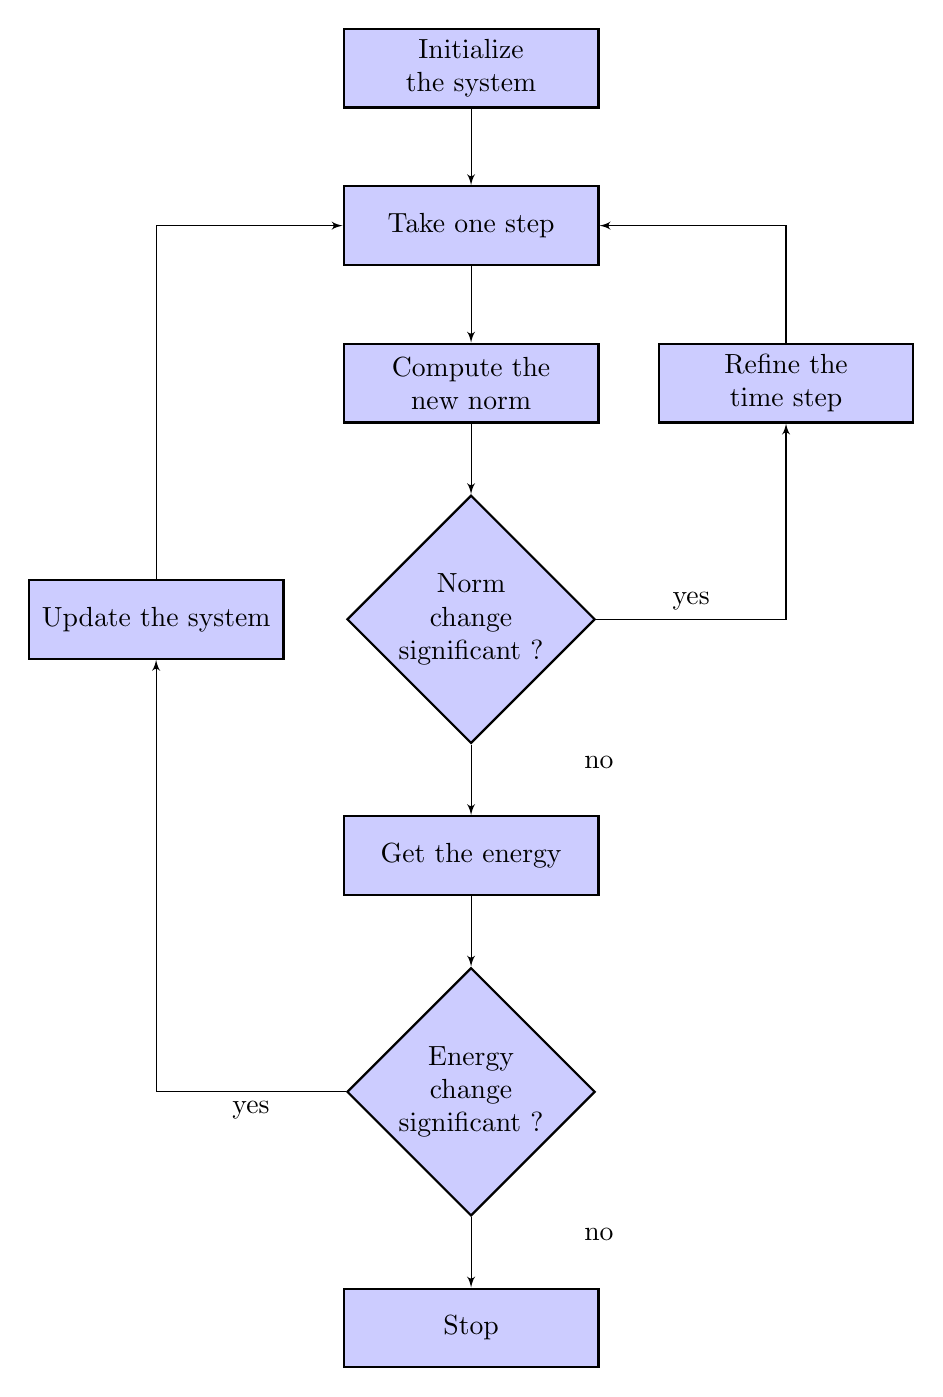
\begin{tikzpicture}[auto,text width=3cm,node distance=2cm,text centered,
	block/.style={rectangle,draw=black,fill=blue!20,thick,minimum height=1cm},
	test/.style={diamond,draw=black,fill=blue!20,thick,inner sep=0pt,text width=2cm},
	line/.style={draw,-latex'}]
\node[block] (input) {Initialize the system};
\node[below of=input,block] (step) {Take one step};
\node[below of=step,block] (normalize) {Compute the new norm};
\node[right of=normalize,block,node distance=4cm] (refine) {Refine the time step};
\node[below of=normalize,test,node distance=3cm] (test) {Norm change significant ?};
\node[left of=test,block,node distance=4cm] (update) {Update the system};
\node[below of=test,block,node distance=3cm] (energy) {Get the energy};
\node[below of=energy,test,node distance=3cm] (test2) {Energy change significant ?};
\node[below of=test2,block,node distance=3cm] (output) {Stop};
\path[line] (input) -- (step);
\path[line] (step) -- (normalize);
\path[line] (normalize) -- (test);
\path[line] (test) --node[near start] {no} (energy);
\path[line] (test) -|node[near start] {yes} (refine);
\path[line] (refine) |- (step);
\path[line] (energy) -- (test2);
\path[line] (test2) --node[near start] {no} (output);
\path[line] (test2) -|node[near start] {yes} (update);
\path[line] (update) |- (step);
\end{tikzpicture}
\caption{Chart flow of the imaginary time propagation algorithm. Detail of one pass.}
\end{center}
\end{figure}

\appendix
\chapter{Getting more by using scripts}
\end{document}